% Data Model
\begin{figure}[htb]
    \centering
    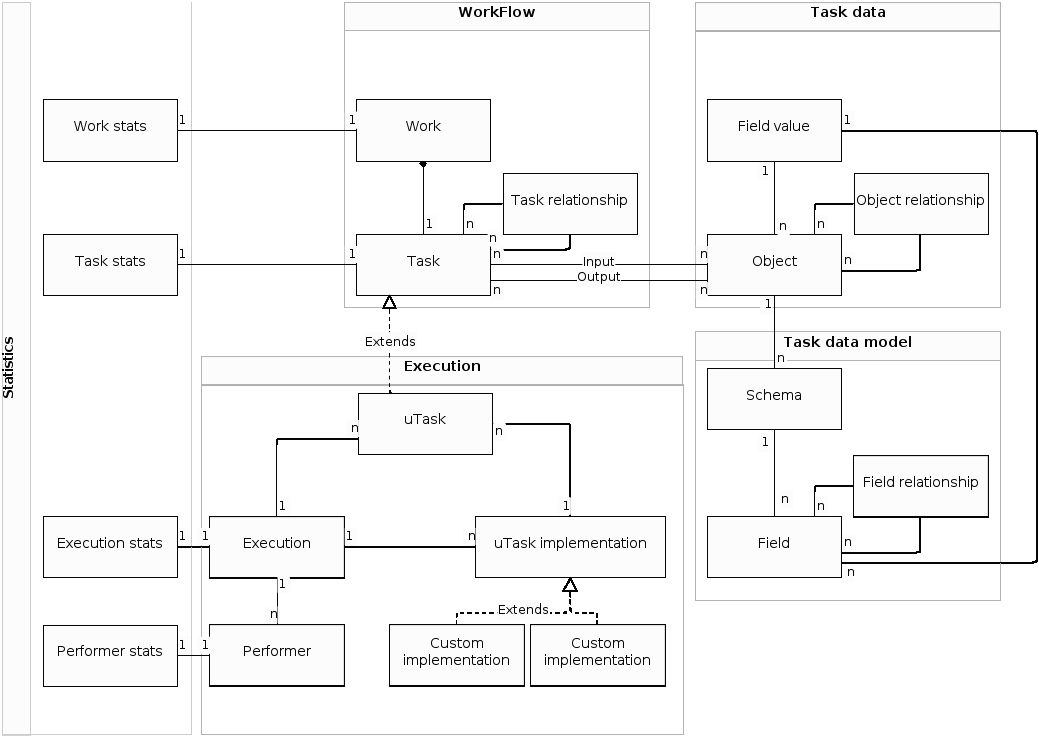
\includegraphics[width=\columnwidth]{DataModel}
    \caption{Data Model.}
    \label{fig:data-model}
\end{figure}
In this section, we define the \emph{Data model} of the System. All the components
used in the \emph{Architectural model} are based on this model and all it's.
As can be seen in \autoref{fig:data-model} the \emph{Data model} is composed of
5 parts that together compose a basic human/automatic computation platform.

\begin{description}
	\item[The WorkFlow] contains the all the information about a \emph{Work},
    including how is composed, in terms of Task, and the relations that
    intercour between two or more Task.

    \item[The Task Data Model] contains the actual data structure for each Task
    or Work.

    \item[The Task Model] contains all the data assocated to a Task or Work.

    \item[The Task Execution] focus on the actual execution step for each Task,
    providing information on wich implementation to use according to a specific
    Performer.

    \item[Statistics] provide all the statistics associated to the Work
    lifeclycle, from the creation to the execution.
\end{description}


\begin{figure}[htb]
    \centering
    
\includegraphics[width=0.75\columnwidth]{ConceptualModel}
    \caption{Conceptual organization of Work, Task and \utask{}.}
    \label{fig:conceptual-model}
\end{figure}

% task con custom proiperties in modo da configurare i runtime

% Step su come funziona la creazione di un task

% Schema type?
% Input data can be associated with a set of Properties, i.e. name-values pairs that have a domain-specific meaning (e.g. the validation status of a given Tweet to be analysed)


% Strategies???

\subsection{WorkFlow}
The WorkFlow embodies all the data associated to the \emph{flow} of Task
that need to be executed in order to complete a \textbf{Work}. As an example
consider image tagging with tag validation as a \emph{Work}, to complete this
we need to perform a few steps:
\begin{enumerate}
    \item Let the user tag an image
    \item Gather the result tags associated to an image
    \item Let some different validate the tags for the image
    \item Gather the validation result
    \item Output the validated tag
\end{enumerate}
As one can notice this \emph{Work} is subdivided in two main steps, the first
when we gather a seet of tag from the users, the second  when these tags are
validated. These tow steps are human computation Task that are part of the
\emph{Work} of image tagging and validation.

\subsubsection{The Work}
The Work represent the main goal of the \emph{Requester} and it's defined by:
\begin{itemize}
    \item A \textbf{Name} that identifies the Work.

    \item \textbf{Contraints} definied by the \emph{Requester} used to prioritize
    the Work among the others (e.g. Due date, Perormer skills, Max execution time).
    % TODO Spiega cosa cazzo vuol dire

    \item \textbf{Input} data, defined by a \emph{Schema}. To keep the model as
    general as possible no assumption are made on the \emph{Schema} type
    (relational, graph, etc.).
    \item \textbf{Output} data, defined as an extension of the input schema
    (sharing the same schema type).

    \item A set of \textbf{Task}. Their orchestration is made at design time,
    specifing a \emph{Flow}
\end{itemize}







\subsubsection{The Flow}
The Flow describes how the \emph{Task} are connected (organized) to fullfill the
rewuirements of a \emph{Work}. In a Flow we can use control structures and
\emph{Variables}. The control structures availabe are:
\begin{description}
     \item[Sequence:] represent the normal flow of an application where one
     operation is executed after the previous is completed.
     \item[Choice:] give the possibility to made choice according to one, or
     more, \emph{Variables}.
     \item[Loop:] Allow to execute some steps multiple times, according to a
     predefined value or a \emph{Variable}.
     \item[Parallel:] the steps of the flow are not executed in \emph{Sequence},
     allowing the parallelization of some steps.
 \end{description} 
The \emph{Variables} can be predefined or computed during the Flow execution to
change the behaviour of the Flow itself. For instance a variable can decide
wheter to execute a loop or not or even decide what control sequence to use in
the next steps.






\subsubsection{The Task}
The Task is the kernel of the whole system, it represent an activity, tipically
focusing on a purpose. A Task is characterized by:
\begin{itemize}
    \item A \textbf{Name} that identifies the Task.

    \item \textbf{Input} data, with a \emph{Schema}. Usually the \emph{Schema}
    of a Task is a projection of the \emph{Schema} of a \emph{Work}.
    \item \textbf{Output} data, with a \emph{Schema} that is an exetension of
    the input \emph{Schema}.

    \item A Task \textbf{type}\footnote{An assumption is made to make the list fit
    all the possible abstract task our System is able to handle.}
    defining, at abstract level, what kind of data manipulation will be performed
    by a Task. These categorization are taken from \cite{paperboz}, here are a
    few:
        \begin{itemize}
            \item Like
            \item Order
            \item Classify
            \item Add
            \item \omissis
        \end{itemize}
    \noindent Each Task type is defined by:
        \begin{itemize}
            \item I/O relationship, defining, at abstract level, how the Task
            transforms the data and the schema.
            \item A default implementation.
        \end{itemize}

    \item A \textbf{Status} encoding the current state of the Task. A Task, can
    have only one of the following statuses at point of its lifecycle:
        \begin{itemize}
            \item \emph{Planning-Input}: the Task has been created, have a
            \emph{Schema} and \emph{Object data} associated and a defined Task
            \emph{type}.

            \item \emph{Planning-\utask{}}: a set of \utask{} has been associated
            to the Task.
            
            \item \emph{Planning-Assignment}: a set of \emph{Performers} has
            been selected to execute the \utask{}.
            
            \item \emph{Wait}: Task planned, \utask{} ready for executiuon.
            
            \item \emph{Running}: \utask{} are running.
            
            \item \emph{Ended}: all the \utask{} have completed their execution.
        \end{itemize}
    
    \item A set of \textbf{Subscriber}s able to recieve updates on the Task
    execution.

    \item A set of \textbf{Execution constraints} used for priortizing the Task
    among others or to modify the standard behaviour of the task to fullfill
    these constraints. The availbale constraints are:
        \begin{itemize}
            \item Maximum execution time
            \item Due date
            \item TODO others
        \end{itemize}

    \item \textbf{Configuration data}, provided as \ac{JSON}. For instance the
    classes we want to use in a calssification Task.

    \item \textbf{\utask{}}s TODO????.
    % i.e. instances of the concrete Task assigned to one or more Performers, to be performed on one or more input objects.

    \item An \textbf{Aggregation} function, in charge of collecting the \utask{}
    results and generating the Task output.
    
    \item \textbf{\utask{} planning} strategy, in charge of defining how many
    \utask{} create for a given Task and associate the right portion of input
    data to such \utask{}. For example total disjunction, redundancy, partial
    overlap, etc.
    
    \item \textbf{Performer assignment} strategy able to assign \emph{Performers}
    to \utask{}. Some strategies can be: manual, random, most reliable, etc.

    \item \textbf{\utask{} implementation} strategy in charge of routing the
    correct \utask{} implementation for each \utask{} execution. The routing
    can be done according to the \emph{user-agent} (e.g. Browser) or to the 
    \emph{user profile} or even \emph{fixed} for all.

    \item A \textbf{Task planning} wich embodies the funcitonalities of
    \emph{\utask{} planning} strategy, \emph{Performer assignment} strategy and
    \emph{\utask{} implementation} strategy deciding the logic behind the
    invocation of those strategies.

    \item A \textbf{Task control} strategy able to control the status of the
    Task and if needed perform corrective actions.

    \item An \textbf{Emission policy} specifing wich \emph{Subscriber} need to
    be notified of a Task change in \emph{Status}.
\end{itemize}











\subsection{Task Data Model}
The Task Data Model contains all the data related to the description of the
\emph{Schema} of the data of a Work/Task. This model resembles a the
\emph{metadata} of the actual data of the Work/Task defining all the fields
and their type according to a \emph{Schema}.


\subsubsection{The Schema}
The Schema contains all the information related to the data structure of a
Work/Task, and its defined by:
\begin{itemize}
    \item A \textbf{Name} that identify the Schema among the others.

    \item A set of \textbf{Field}s that compose the actual schema of the data. 
    
    \item A list of \textbf{Object}s associated to this \emph{Schema}, these
    objects represents the actual data associated to the Work/Task.
\end{itemize}



\subsubsection{The Field}
The Field represent the definition of a Field in a \emph{Schema}, with all the
properties that define if the field is calculated, derived, etc. The Field is
defined by:
\begin{itemize}
    \item A \textbf{Name} that identify the Field.
    
    \item A \textbf{type} definig the type of the data that this field contains.
    i.e. \code{string}, \code{number}, etc.

    \item A set \textbf{related fields} that defines how this field is composed.
    TODO ???
    
    \item A \textbf{relation} that specifies which type of relation occurs among
    the \emph{related fields}.

    \item The list of \textbf{data} of in terms of the associated \emph{Field
    values}
\end{itemize}





\subsection{Task Data}
The Task Data contains the actual data instance for each Task, defined in the
\emph{Schema}. All the data are contained in a \emph{Object} that represent the
the instance of the Task data (e.g. A row of the Task Data table). Due to the
metadata-like model of the System, we need to store all these information into
a separate table and use the \emph{Object} as a simple reference table.

\subsubsection{The Object}
The Object contains the actial data value as reference to field value instances;
it's composed by:
\begin{itemize}
    \item A \textbf{Name}.
    \item A list of field values \textbf{data}.
    \item TODO ??
\end{itemize}


\subsubsection{The Field Value}
The Field Value contains the data associated to a particular field, defined in
the metedata model. It's defined by:
\begin{itemize}
    \item An \textbf{Object} that define tho what \emph{Object} they refer to.
    \item The \textbf{Field} to wich the datta belongs.
    \item TODO ???
\end{itemize}







\subsection{Task Execution}
The Task Exection embodies all the information relative to the actual exection
of the code. The majority of these data belongs to the \textbf{Execution layer}
thus can be phisically located into another piece of software in charge of the
execution of the code.


\subsubsection{\utask{}}
The \utask{} is the implementation of a Task that insist on a specific subset
of data of the Task. Can be also considered as an activity assigned to one or
more Performers. It is defined by:
\begin{itemize}
    \item A \textbf{Name}.
    
    \item A list of \textbf{Execution}, representing the actual activities
    performed by a \emph{Performer}
    
    \item A set of \textbf{Execution constraints}.
    
    \item \textbf{Input} data, as a subset of the Task input data.
    
    \item \textbf{Output} data, with the same schema as the related Task output
    data.
    
    \item A list of \textbf{Properties}, defined as name-value pairs, having
    domain specific meaning. 
    
    \item One or more \textbf{\utask{} implementation}.
\end{itemize}







\subsubsection{The Execution}
The Execution is related to one \emph{Performer} that need to compute a \utask{}.
An Execution is defined by:
\begin{itemize}
    \item a \textbf{Status} telling the status of the execution of the \utask{},
    the available statuses are:
    \begin{itemize}
        \item \emph{running}
        \item \emph{suspended}
        \item \emph{idle}
        \item \emph{ended}
    \end{itemize}

    \item A set of \textbf{Execution data} provided as \ac{JSON} object.

    \item A \utask{} \textbf{Implementation}
\end{itemize}







\subsubsection{\utask{} implementation}
The \utask{} Implementation is the actual application logic and presentation
delivered to a \emph{Performer} to run a \utask{}. The System provides a default
implementation according to the Task type, in addition, a \emph{Requester} can
specify one or more Custom implementations, in order to obtain more control over
the execution process.








\subsubsection{Performer}
A Performer is a human being able to execute one or more \utask{}. The performer is characterized by a set of attributes such as:

\begin{itemize}
    \item A \textbf{Name}
    \item \textbf{Demographic} information
    \item \textbf{Performance} information
    \item \textbf{Trustworthiness}
    \item \textbf{Social properties}
\end{itemize}






\subsection{Statistics}
This Statistics model contains all the information related to the Task profiling
and statistics used to tweak the performance of a Task, or used by components
(like the \emph{Task controller}) to take decision on the Task flow. In this
model are contained data about \emph{Work}, \emph{Task}, \emph{\utask{}},
\emph{Performer}, etc. The data contained in these tables can be:
\begin{itemize}
    \item \textbf{Creation date}
    \item \textbf{Total execution time}
    \item \textbf{Average number of \emph{Performer}s/h}
    \item \textbf{Last execution}
    \item etc.
\end{itemize}
